\documentclass[11pt]{article}
\usepackage[margin=2.5cm]{geometry}
\usepackage{booktabs}
\usepackage{graphicx}
\usepackage{amsmath}
\usepackage{textcomp}
\usepackage[hidelinks]{hyperref}

\title{Ablation Study Results}
\date{}

\begin{document}
\maketitle

\section*{Overview}

We systematically ablate individual model components to identify which mechanisms
are necessary for the emergence of rhythmicity in Group~2 (the non-rhythmic
group).  Each condition was run with 5 independent seeds and 200 permutations
for the rhythmicity test.  We report the sine-fit amplitude $A$ and the
permutation $p$-value for Group~2.

%% ── Figure 1: Single-factor bar chart ──────────────────────────────────────
\begin{figure}[ht]
  \centering
  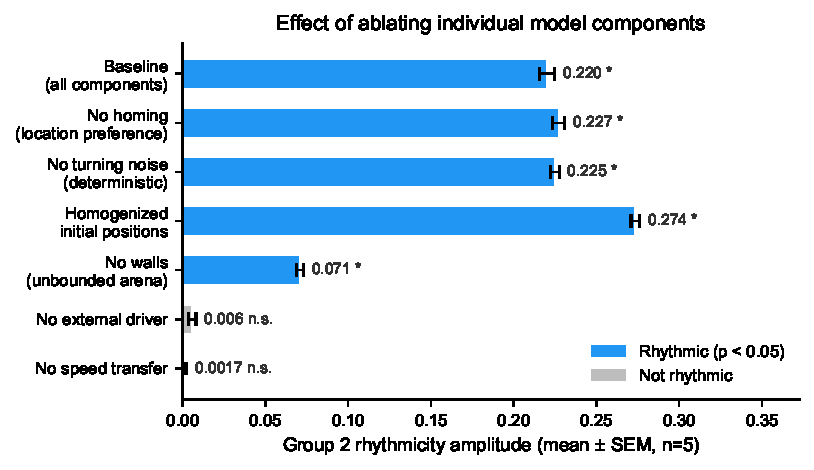
\includegraphics[width=\textwidth]{ablation_single_factor.pdf}
  \caption{Effect of ablating individual model components on Group~2
    rhythmicity amplitude (mean $\pm$ SEM, $n{=}5$ seeds).
    Speed transfer is the only component whose removal eliminates Group~2
    rhythmicity entirely ($A_2 \approx 0.002$, $p = 0.36$).
    Walls have a secondary amplifying effect, reducing $A_2$ from $0.223$
    to $0.059$ (confinement increases contact rate).
    Homing and turning noise have negligible effects.
    Homogenizing initial positions slightly \emph{increases} transfer
    ($A_2 = 0.234$), since mixing groups spatially produces more
    early inter-group contacts.}
  \label{fig:single-factor}
\end{figure}

%% ── Figure 2: Factorial heatmap ────────────────────────────────────────────
\begin{figure}[ht]
  \centering
  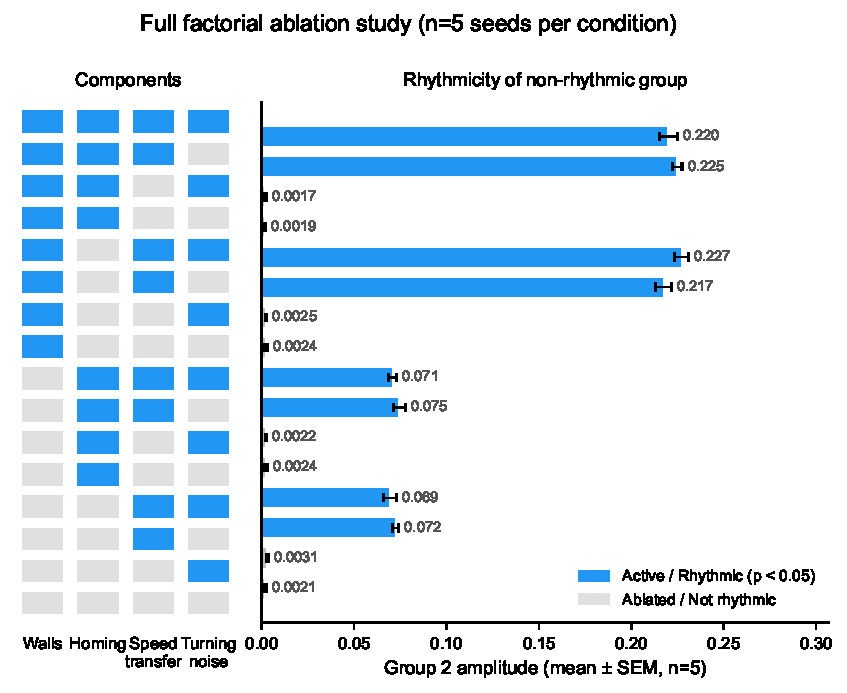
\includegraphics[width=\textwidth]{ablation_factorial_heatmap.pdf}
  \caption{Full $2^4$ factorial ablation over four structural components
    ($n{=}5$ seeds per condition).  Left: blue squares indicate the
    component is active; grey indicates it has been ablated.  Right:
    Group~2 amplitude.  Whenever speed transfer is ablated (grey in
    the third column), Group~2 amplitude collapses to near zero
    regardless of other component states.}
  \label{fig:factorial}
\end{figure}

%% ── Table ──────────────────────────────────────────────────────────────────
\begin{table}[ht]
\centering
\caption{Ablation study: effect of removing individual model components on rhythmicity transfer (mean $\pm$ SEM across $n{=}5$ independent seeds). $A_1$ and $A_2$ are the fitted sinusoidal amplitudes of the Group~1 (forager) and Group~2 (hive bee) mean speed time series, respectively. $\Delta\phi$ is the phase lag of Group~2 relative to Group~1 in degrees, and $p_2$ is the permutation-test $p$-value for Group~2 rhythmicity (200 permutations). Simulations used density factor $d{=}1.0$, day duration $T_{\mathrm{day}}{=}100$~steps, and decay rate $\gamma{=}0.8$. Speed transfer is the sole essential mechanism; walls provide secondary amplification by confining agents and increasing contact rates.\textsuperscript{a}}
\label{tab:ablation}
\small
\begin{tabular}{@{}lcccc@{}}
\toprule
\textbf{Condition} & $A_1$ & $A_2$ & $\Delta\phi$ (\textdegree) & $p_2$ \\
\midrule
  Baseline (all components) & $1.25 \pm 0.00$ & $0.220 \pm 0.005$ & $14.8 \pm 0.6$ & $<$0.01 \\
  No speed transfer & $1.25 \pm 0.00$ & $0.0017 \pm 0.0008$ & --- & 0.65 \\
  No homing (location preference) & $1.25 \pm 0.00$ & $0.227 \pm 0.004$ & $12.7 \pm 1.3$ & $<$0.01 \\
  No walls (unbounded arena) & $1.25 \pm 0.00$ & $0.071 \pm 0.002$ & $20.2 \pm 4.3$ & $<$0.01 \\
  No turning noise & $1.25 \pm 0.00$ & $0.225 \pm 0.003$ & $14.8 \pm 0.6$ & $<$0.01 \\
  No external driver & $0.01 \pm 0.00$ & $0.006 \pm 0.002$ & --- & 0.36 \\
  Homogenized initial positions & $1.24 \pm 0.00$ & $0.274 \pm 0.003$ & $8.6 \pm 1.0$ & $<$0.01 \\
  No homing + no speed transfer & $1.25 \pm 0.00$ & $0.0025 \pm 0.0002$ & --- & 0.31 \\
  No walls + no speed transfer & $1.25 \pm 0.00$ & $0.0022 \pm 0.0003$ & --- & 0.42 \\
  No walls + no homing & $1.25 \pm 0.00$ & $0.069 \pm 0.004$ & $7.7 \pm 1.6$ & $<$0.01 \\
  No walls, homing, or speed transfer & $1.25 \pm 0.00$ & $0.0031 \pm 0.0005$ & --- & 0.21 \\
\bottomrule
\end{tabular}

\vspace{2pt}
{\scriptsize \textsuperscript{a}Phase shift omitted where Group~2 rhythmicity was not significant ($p \geq 0.05$).}
\end{table}


%% ========================================================================
\section*{Supplementary: Parameter Sensitivity}
%% ========================================================================

To assess the robustness of the speed-transfer model, we performed
single-parameter sweeps over the three main tunable parameters: agent density
$d$, day duration $T_{\mathrm{day}}$, and decay rate $\gamma$.  In each sweep
one parameter is varied while all others are held at their baseline values
($d{=}1.0$, $T_{\mathrm{day}}{=}100$~steps, $\gamma{=}0.8$); each condition
is evaluated with $n{=}5$ independent seeds and 200~permutations.

\subsection*{Summary of parameter effects}

\paragraph{Density ($d$).}
The density factor scales the number of agents in the arena and thereby controls
the availability of interaction partners.  Higher density increases the rate
of inter-group contacts, which leads to faster build-up of rhythmicity in
Group~2 (larger $A_2$) and correspondingly shorter propagation delays (smaller
$\Delta\phi$).  Both effects are monotonic: $A_2$ increases
approximately linearly from $0.07$ at $d{=}0.25$ to $0.37$ at $d{=}3.0$,
while $\Delta\phi$ decreases from ${\sim}17\text{\textdegree}$ to
${\sim}9\text{\textdegree}$ (Fig.~\ref{fig:sensitivity-density}).

\paragraph{Day duration ($T_{\mathrm{day}}$).}
The day duration sets the number of simulation steps per light--dark cycle.  A
longer cycle provides more samples per day, making the temporal resolution
finer, but it also means the exponential decay $\gamma$ is applied more times
per day---the effective per-day memory is $\gamma^{T_{\mathrm{day}}}$, which
becomes negligibly small for large $T_{\mathrm{day}}$ (e.g.\
$0.8^{400}\!\approx\!10^{-39}$).  In practice, amplitude is largely invariant
to day duration ($A_2 \approx 0.22$ for $T_{\mathrm{day}} \geq 75$),
confirming that the steady-state transfer signal does not depend on temporal
resolution.  By contrast, phase lag scales inversely with $T_{\mathrm{day}}$:
$\Delta\phi \approx 31\text{\textdegree}$ at $T_{\mathrm{day}}{=}50$ down to
$\Delta\phi \approx 2\text{\textdegree}$ at $T_{\mathrm{day}}{=}800$
(Fig.~\ref{fig:sensitivity-duration}).  This relationship arises because the
propagation delay is approximately constant in absolute time steps; as the
cycle length increases, this fixed delay represents a progressively smaller
fraction of the full $360\text{\textdegree}$ cycle.

\paragraph{Decay rate ($\gamma$).}
The decay rate implements a leaky memory of past speed transfers: at each time
step, the accumulated speed-transfer signal is multiplied by $\gamma$,
so $\gamma{=}0$ corresponds to no memory (only instantaneous interactions)
and values approaching~$1$ retain nearly all past information.
Amplitude increases monotonically with $\gamma$ ($A_2 \approx 0.06$ at
$\gamma{=}0$ to $A_2 \approx 0.30$ at $\gamma{=}0.9$), because longer
memory allows the rhythmic signal to accumulate across multiple interactions
(Fig.~\ref{fig:sensitivity-decay}).  Crucially, rhythmicity transfer remains
significant ($p < 0.01$) even at $\gamma{=}0$, demonstrating that the basic
mechanism does not require temporal integration.  Phase lag also increases
substantially with $\gamma$, approximately tripling from
$\Delta\phi \approx 7\text{\textdegree}$ at $\gamma{=}0$ to
$\Delta\phi \approx 21\text{\textdegree}$ at $\gamma{=}0.9$.  This is
because the accumulated memory acts as inertia: at high~$\gamma$, an agent's
speed is heavily influenced by interactions from many previous steps, so it
takes longer for the current phase of the driving rhythm to override the
historical signal, delaying the response of Group~2.

\subsection*{Figures}

%% ── Figure S1: Density sweep ───────────────────────────────────────────────
\begin{figure}[ht]
  \centering
  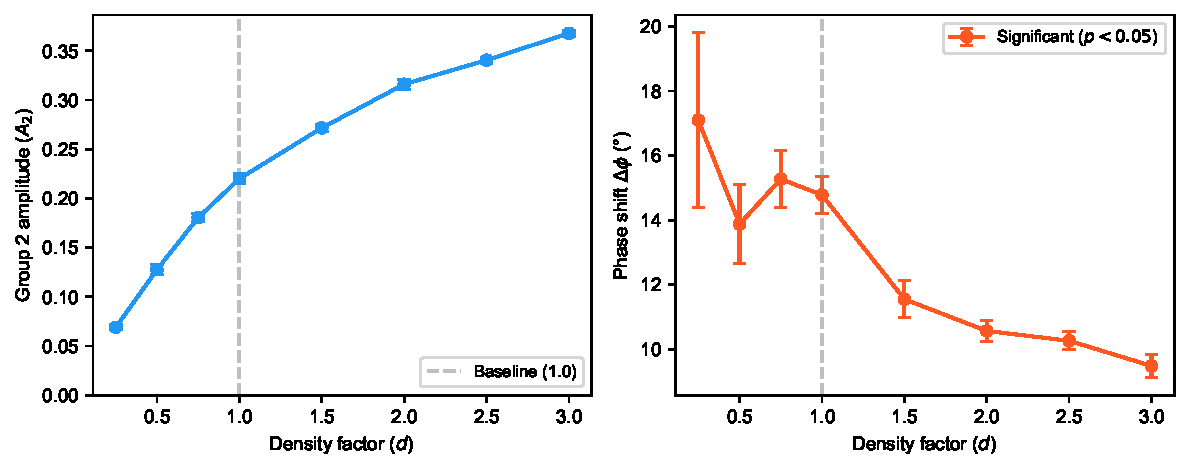
\includegraphics[width=\textwidth]{sensitivity_density.pdf}
  \caption{Sensitivity to agent density ($d \in [0.25, 3.0]$,
    $T_{\mathrm{day}}{=}100$, $\gamma{=}0.8$).
    \textbf{Left:} Group~2 amplitude $A_2$ increases monotonically with density.
    \textbf{Right:} Phase lag $\Delta\phi$ decreases with density, as more
    available interaction partners accelerate signal propagation.
    Dashed line marks the baseline ($d{=}1.0$).}
  \label{fig:sensitivity-density}
\end{figure}

%% ── Figure S2: Day duration sweep ──────────────────────────────────────────
\begin{figure}[ht]
  \centering
  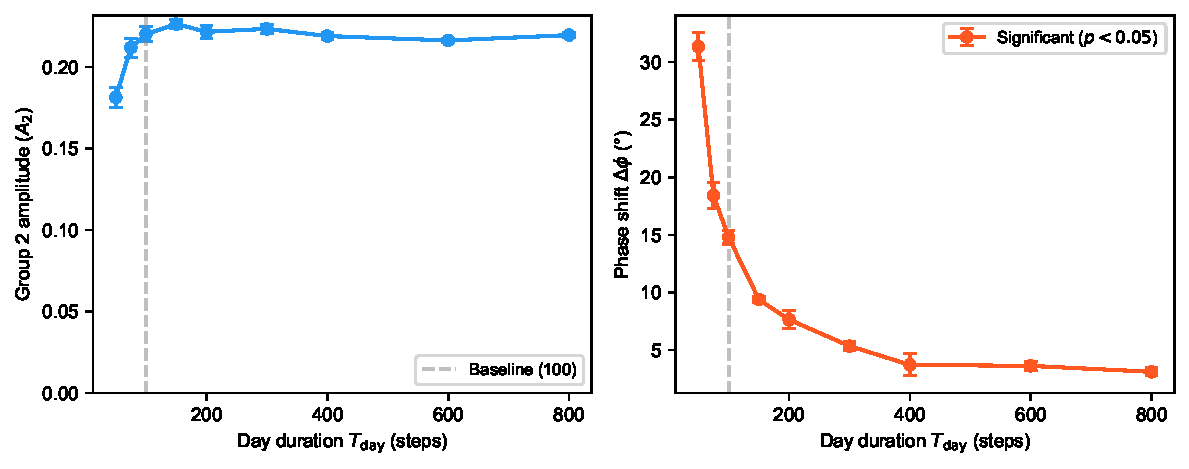
\includegraphics[width=\textwidth]{sensitivity_day_duration.pdf}
  \caption{Sensitivity to day duration ($T_{\mathrm{day}} \in [50, 800]$~steps,
    $d{=}1.0$, $\gamma{=}0.8$).
    \textbf{Left:} Amplitude is nearly constant for $T_{\mathrm{day}} \geq 75$.
    \textbf{Right:} Phase lag scales inversely with day duration, consistent
    with a fixed propagation delay measured in steps.
    Dashed line marks the baseline ($T_{\mathrm{day}}{=}100$).}
  \label{fig:sensitivity-duration}
\end{figure}

%% ── Figure S3: Decay sweep ─────────────────────────────────────────────────
\begin{figure}[ht]
  \centering
  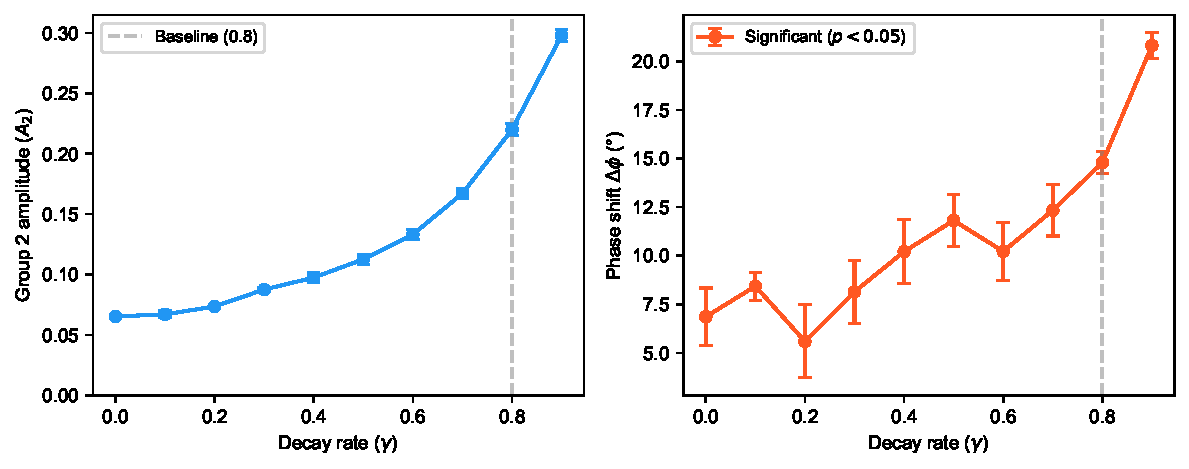
\includegraphics[width=\textwidth]{sensitivity_decay.pdf}
  \caption{Sensitivity to decay rate ($\gamma \in [0.0, 0.9]$,
    $d{=}1.0$, $T_{\mathrm{day}}{=}100$).
    \textbf{Left:} Amplitude increases with $\gamma$ as longer memory
    amplifies the accumulated signal.  Importantly, transfer is significant
    ($p < 0.01$) even at $\gamma{=}0$.
    \textbf{Right:} Phase lag increases approximately threefold from
    $\gamma{=}0$ to $\gamma{=}0.9$, reflecting inertia from accumulated
    memory.  Dashed line marks the baseline ($\gamma{=}0.8$).}
  \label{fig:sensitivity-decay}
\end{figure}

\end{document}
